\section*{Opgave A}

\begin{figure}[H]
    \centering
    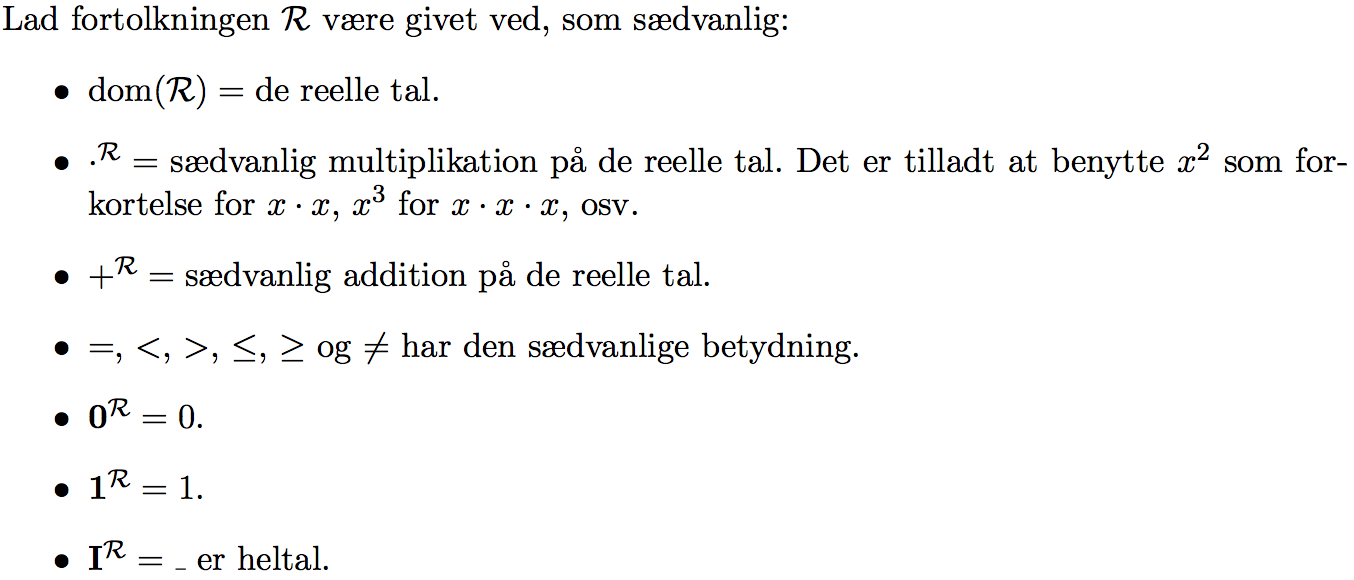
\includegraphics[width=1.0\textwidth]{opgA/opgA.png}
    \label{fig:opgA}
\end{figure}

Hver af følgende udsagn skrives med første-ordens prædikatslogik i fortolkningen $\mathcal{R}$. Når der optræder mere end ét reelt tal, bruger vi $x$ og $z$. $x$ er et vilkårligt reelt tal, $z$ er et reelt tal, vi giver egenskaben at være heltal med notationen $I(z)$. 

\begin{enumerate}
    \item Der findes et reelt tal som ikke er et heltal
    
        \begin{equation*}
            \exists x(\neg I(x))
        \end{equation*}
        
        \begin{flushright}
            Sandt, da ikke alle reelle tal er heltal, fx $\pi$ og $\frac{1}{2}$.
        \end{flushright} 
    
    \item Der findes et reelt tal som er større end alle heltal.
    
        \begin{equation*}
            \exists x \forall z \big(I(z) \rightarrow \left( x>z\right)\big)
        \end{equation*}
        
        \begin{flushright}
            Falskt, da der ingen øvre grænse er for heltal.
        \end{flushright} 
        
        
    \item Ethvert positivt heltal er kvadratet af et negativt reelt tal.
    
    Sætningen antages ækvivalent med: \\ "For alle positive heltal $z$, findes et negativt reelt tal $x$ der kvadreret giver $z$"
    
    \begin{equation*}
            \forall z \Big(\big((z>0) \wedge I(z)\big) \rightarrow \exists x\big((x<0) \wedge (x^2 = z)\big)\Big)
        \end{equation*}
        
        \begin{flushright}
            Sandt, da $\pm\sqrt{z} \in \mathbb{R}$ for $z \in \mathbb{Z}$, og kvadratet af et negativt reelt tal er positivt. Eksempel: heltallet 3 kan findes ved $(- \sqrt{3})^2$.
        \end{flushright} 
        
        
\end{enumerate}